\documentclass{article}
\usepackage{amsmath}
\usepackage{hyperref}
\usepackage{graphicx}

\hypersetup{
	colorlinks=true,
	linkcolor=blue,
	filecolor=magenta,      
	urlcolor=blue,
	pdfpagemode=FullScreen,
}

\begin{document}


\subsection{Abstract}	
The aim of this document is to outline the recreation of the CSTR model created in this \href{}{paper} in an open-source framework. The main goals of this project are:
\begin{itemize}
	\item Successfully recreate the model and steady-state results in Julia
	\item Recreate some incipient fault scenarios
	\item Generate a data set that can subsequently be used for further fault detection
\end{itemize}

\subsection{Introduction}

\href{https://dspace.lib.cranfield.ac.uk/bitstream/handle/1826/13055/Canonical_variate_dissimilarity_analysis-2018.pdf?sequence=4}{Pilario \& Cao (2018)} developed a model for the detection of incipient faults. To test their model, they tested it against a simulation model of a CSTR that was modified to take into account the intricacies of real-time data. This includes things such as parameter mismatch, sensor drift, Gaussian noise and other phenomena that cause a process to deviate from theoretically ideal behaviour. The benefit in doing this is that they can successfully test their fault detection model against both normal, steady-behaviour and against simulations where a fault has been introduced. The aim of the fault detection model is naturally to minimize the occurrence of false positives in normal behaviour and minimize the lag in detection during faulty scenarios. 

The CSTR model in this paper was modelled in Simulink is available \href{https://uk.mathworks.com/matlabcentral/fileexchange/66189-feedback-controlled-cstr-process-for-fault-simulation}{online} and can be subsequently used for data set generation for anyone with a MATLAB/Simulink license. However, this process should be simple enough to be sufficiently easy to solve with available open source tools. Julia lang in particular has several packages that can be used for the solution of differential equations with easy to follow documentation \href{https://diffeq.sciml.ai/stable/}{here}. 

Furthermore, there is currently a crisis in Science academia in general where relatively few people strive to reproduce the results that are published in peer-review journals. Pilario \& Cao (2018) have written a very good paper that showcases all the model details that can be used for the reproduction of its results. As such, this is a good candidate paper to try to reproduce without having to ask the authors up front for any missing data. 



As such, there are multiple aims in this project:


\begin{itemize}
	\item To recreate the CSTR results presented in the paper for steady and some incipient fault scenarios
	\item To test the use of the Julia programming language in solving this kind of use case
	\item To generate a data set that can be subsequently used by others for the testing of incipient faults
\end{itemize}

I hope to outline my approach so that it is as easy to follow alongside the code that can be used by anyone to recreate the results. 

\subsection{Methodology}

We start with a model schematic of the physical process (shown in Figure \ref{fig1}) and the differential equations that describe its dynamics. 
 
\begin{figure}[h]	\centering
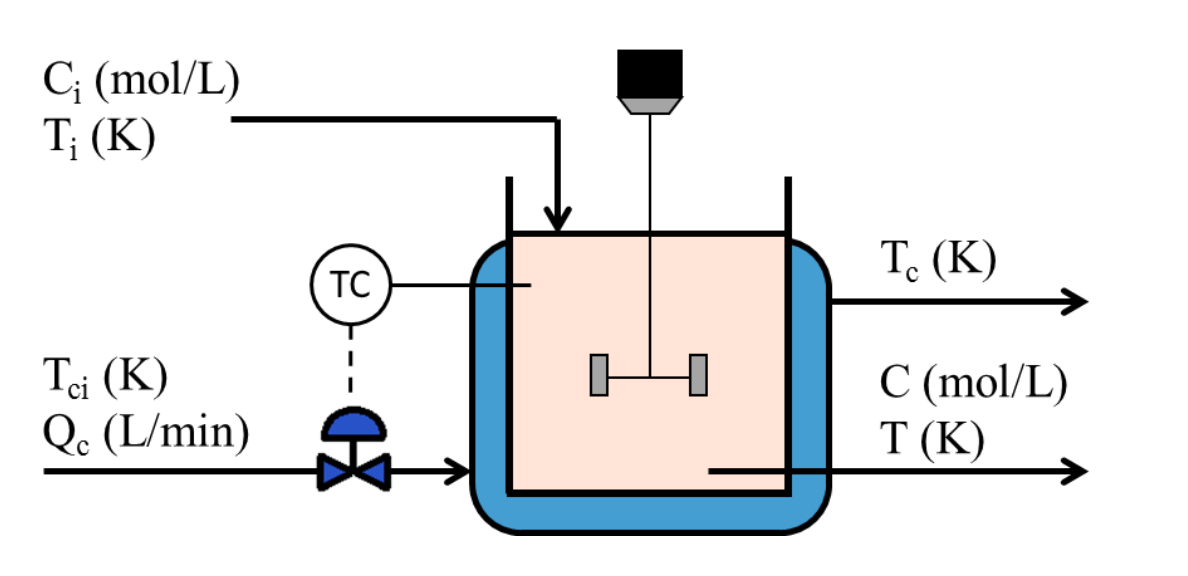
\includegraphics[width=\textwidth]{img/CSTR_schematic.png}
\caption{Schematic of a CSTR model from Pilario \& Cao (2018)}
\label{fig1}
\end{figure}



\end{document}